\section{Организационно-экономическая часть}

\subsection{Описание разрабатываемого продукта}
\begin{par}
Разработанное устройство --- <<цифровые часы с будильником>> позволяют отображать
текущее время на большом графическом жидкокристалическом дисплее. Удобным для
потребителя методом производить ввод времени срабатывания будильника.
Устройство, позволяет не пребегая к перепрограммированию внутренней памяти, менять
мелодию звуковой сигнализации. А так же производить синхронизацию текущего времени
с высокоточным удалённым сервером времени.
\end{par}

\begin{par}
К достоинству системы так же можно отнести то, что она реализована в соотвествии с манифестом
разработчиков открытого аппаратного обеспечения, что может прозволить повысить качество потребительских
характеристик устройства за счёт привлечения сообщества разработчиков открытого аппаратного
обеспечения. Так устройство или его часть может быть использовано в других ещё более
совершенных бытовых устройствах разрабатываемых сторонними производителями.

\begin{figure}[h]
	\center{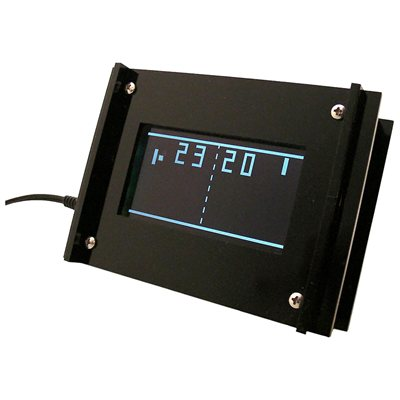
\includegraphics[bb=0 0 300 300, clip, scale=0.8]{adafruit.png}}
	\caption{Adafruit Monochron Open Source Clock kit}
	\label{img:adafruit}
\end{figure}

\end{par}

\subsection{Исследование существующих программных продуктов}
\begin{par}
Фактически на текущий момент на рынке существует только один аналог разработанного
утройства ---  Adafruit Monochron Open Source Clock kit.
Сравнительный обзор устройств представлен в таблице \ref{table:compare}.
\end{par}


\begin{par}
\begin{table}
\caption{Сравнение ''Цифровые часы с будильником'' и ''Adafruit''}
\begin{tabular}{|l|p{4cm}|p{4cm}|}
\hline{}
Характеристика & Цифровые часы с\linebreak{} будильником & Adafruit \\
\hline{}
Микроконтроллер & новое поколение AVR Xmega --- atxmega32a4 & старое семейство контроллеров AVR Mega -- atmega328 \\
\hline{}
ЖКИ & TFT 320x240 & LCD 128x64 \\
\hline{}
Метод ввода & сенсорный экран & кнопочное управление \\
\hline{}
Мелодии будильника & разнообразные мелодии выбираемые пользователем, одна встроенная мелодия & мерцание ЖКИ и звуковая сигнализация пъезоэлектрическим излучателем \\
\hline{}
Синхронизация с сервером времени & присутствует & отсутствует \\
\hline{}
Количество вариантов сборки & 1 & более 10 \\
\hline{}
Ориентировочная цена & 90\$ & 90\$ \\ 
\hline{}
Привлекательное название & отсутствует & присутствует \\ 
\hline
\end{tabular}
\label{table:compare}
\end{table}

Как видно из представленной таблицы, спректированное устройство имеет ряд преимуществт перед
устройством Adafruit. К недостаткам можно отнести только низкое число вариантов сборки устройства,
вызванное малой распространённостью разработанного устройства, что является
следствием не завершёности стадии его проектирования и разработки, а так же отстутствием каких-либо
действий нацеленных на устронение этого недостатка.
\end{par}
\newpage{}

